\documentclass[10pt]{article}
\usepackage{../../local}
\urlstyle{same}

\newcommand{\classcode}{EE 120}
\newcommand{\classname}{Signals and Systems}
\renewcommand{\maketitle}{%
\hrule height4pt
\large{Eric Du \hfill \classcode}
\newline
\large{Lecture Notes} \Large{\hfill \classname \hfill} \large{Chunlei Liu}
\hrule height4pt \vskip .7em
\small{Header styling inspired by CS 70: \url{https://www.eecs70.org/}}
\normalsize
}
\linespread{1.1}

\newcommand{\question}[1]{\textcolor{red}{#1}}
\newcommand{\answer}[1]{\textcolor{green!80!black!}{#1}}
\renewcommand{\comment}[1]{\textcolor{blue!50}{#1}}

\newcommand{\corr}{\mathrm{corr}}
\begin{document}
	\maketitle
	\section{Introduction}
\subsection{Motivations} 
\begin{itemize}
	\item Why study this class?
		\begin{itemize}
			\item Given a "black box" circuit, with input and output leads, we can determine what's within 
				the "black 
				box".
			\item In this particular case, if our black box contains a voltage divider, and the output voltage is given 
				by the equation:
				\[
				v_{\text{out}}(t) = \frac{R_2}{R_1+ R_2}v_{\text{in}}(t)
				\] 
				In principle though, the signal can be anything that we want: for facial recognition software, the input
				signal could be the configuration of the intensity the camera picks up. There's many more we went over, 
				don't really want to write it all down. 
		\end{itemize}
	\item In essence, there's a lot of systems that can be modeled by a system that takes in a signal \( x(t) \), and 
		outputs a signal \( y(t) = f(x(t))\).
		\begin{itemize}
			\item The signals are usually functions of time, location, in any number of dimensions.
			\item The systems does some sort of transformation on an input signal. In particular, we will study 
				linear systems, shift-invariant systems, etc.
				
				We'll talk about mathematical operations that we use to perform these transformations: Fourier, 
				Laplace, Z-transformations, convolutions, correlation, etc.\item 
	\end{itemize}
\end{itemize}
\subsection{Types of Signals}
\begin{itemize}
	\item \textbf{Continuous-time:} signals defined over continuous variables (e.g. position, time). For 
		instance, a signal \( x(t) \) is continuous for our purposes, since time is a continuous variable. 

		Further, because \( t \) is continuous, then \( x \) must also be continuous.  If the signal is differentiable, 
		then the derivative \( \dv{x(t)}{t} \) also exists. 

		\question{\( t \) being continuous does not imply that \( x(t) \) is continuous (e.g. Thomae function),
		but is it true for this class?} 
	\item \textbf{Discrete-Time:} These are signals defined over discrete variables. For instance, if we had 
		\( x[n] \) as a signal, where \( n \) is an integer. 

		We don't have a concept of differentiability, but we can compute the difference: \( x[n] - x[n- 1] \), and 
		talk about that quantity. 
	\item \textbf{Real-Valued:} A signal \( x(t) \) is real-valued if \( x(t) \in \mathbb R \), where \( \mathbb R \) 
		denotes the set of all real numbers. 
	\item \textbf{Complex-Valued:} A signal \( x(t)  \) is complex-valued if \( x(t) \in \mathbb C \), where 
		\( \mathbb C \) denotes the set of complex numbers. 
	\item Note that while we're using the continuous-time notation here, the same concepts apply with discrete-time 
		signals. 

		\begin{itemize}
			\item Quick recap on complex numbers: denoted by \( a + bj \) or \( a + bi \), where \( i \) and \( j \) 
				denote the imaginary unit. 
			\item They are defined as \( i^2 = -1 \) or \( j^2 = -1 \).
			\item \( a \) is the real part, and \( b \) is the imaginary part. 
			\item We can plot these values in the complex plane, using the real and imaginary representation:
				\begin{center}
					\begin{tikzpicture}
						\draw[-stealth, thick] (-3, 0) -- (3, 0) node[above] {real};
						\draw[-stealth, thick] (0, -3) -- (0, 3) node[above right] {imaginary};
						\draw[red] (0, 0) -- (1.8, 1.4) node[above right, black] 
							{\( z = a + bj \) }; 
						\filldraw[red] (1.8, 1.4) circle (2pt); 
						\draw[dashed] (1.8, 1.4) -- (1.8, 0) node[below] {\( a \) };
						\draw[dashed] (1.8, 1.4) -- (0, 1.4) node[left] {\( b \) };
					\end{tikzpicture}
				\end{center}
				Or using the magnitude-phase representation:
				\begin{center}
					\begin{tikzpicture}
						\draw[-stealth, thick] (-3, 0) -- (3, 0) node[above] {real};
						\draw[-stealth, thick] (0, -3) -- (0, 3) node[above right] {imaginary};
						\draw[red] (0, 0) -- node[midway, above left] {\( m \) } (1.8, 1.4) node[above right, black] 
							{\( z = m\cdot e^{j \theta} \) }; 
						\filldraw[red] (1.8, 1.4) circle (2pt); 
						\draw[red] (1, 0) arc (0:37.87:1) node[midway, right]{\( \theta \) };
						\draw[dashed] (1.8, 1.4) -- (1.8, 0) node[below] {\( m \cdot \cos (\theta) \) };
						\draw[dashed] (1.8, 1.4) -- (0, 1.4) node[left] {\( m \cdot \sin (\theta) \) };
					\end{tikzpicture}
				\end{center}
				We represent the magnitude as \( m = |z| \), and the phase angle \( \theta \) is the angle made 
				with the real axis. 
		\end{itemize}
	\item \textbf{Periodic Signal:} Two quantities we'll introduce here: the period \( T \) is the time it takes 
		for the signal to repeat itself. \( T \) is measured in units of time, generally seconds.
		
		The frequency \( f \) is the "inverse" of period, defined by \( f = \frac{1}{T} \). We will also use 
		the angular frequency \( \omega \), defined by \( \omega = \frac{2\pi}{T} = 2 \pi f \). Angular frequency
		is mainly going to be used when we involve complex numbers. We will see:
		\[
		e^{j \omega t} = e^{j (2 \pi f t)} = \cos(2 \pi ft) + i \sin (2 \pi ft)
		\] 
	\item \textbf{Dimensionality:} We will deal with multi-dimensional signals: an example of a 2D signal are images, 
		which determine the color of a pixel based on a row and column. The spaces that we'll be working with are 
		either \( \mathbb R^{n} \) or \( \mathbb C^{n} \). 
\end{itemize}
\subsection{Signal Transformations}
\begin{itemize}
	\item \textbf{Shifts:} Essentially just shifts the signal along one dimension: \( x(t) \to x(t - T) \). \( T \) 
		is some constant. If  \( T > 0 \), then the shift is to the \textit{right}, and if \( T < 0 \) then 
		the shift is to the \textit{left}.
	\item \textbf{Scaling:} We can multiply a signal \( x(t)  \) by some constant \( a \) : \( x(t) \to a\cdot x(t) \).
		If \( a < 1 \), then we shrink \( x(t) \), and if \(  a > 1 \) then we amplify the signal. 
	\item \textbf{Reversal:} Given \( x(t) \), we can "reverse time" by adding a negative to the argument: \( x(t)
		\to x(-t)\). Visually, all we do is flip the signal around the \( y \)-axis.  
\end{itemize}
\subsection{Signal Properties}
\begin{itemize}
	\item \textbf{Even:} Functions which satisfy \( x(t) = x(-t) \). In other words, if we perform a reversal, the 
		signal stays the same.
	\item \textbf{Odd:} Functions which satisfy \( x(t) = -x(-t) \). If we perform a reversal, the signal becomes the 
		negative of itself.
	\item \textbf{Periodic:} If \( T \) is the period, then \( nT \) is also a period for any \( n \in \mathbb Z \).
		However, we will call \( T \) the fundamental period; the smallest \( T \) for which the function 
		repeats. 

		For the function \( \sin(2 \pi ft) \), the fundamental period is \( 1 / f \).  
\end{itemize}
\subsection{Model Functions}
\begin{itemize}
	\item These are called model functions because they're idealized models to analyze. 
	\item \textbf{Heaviside Step function:} For the continuous-time case it's usually modeled by:
		\[
		u(t) = \begin{cases}
			0 & \text{for \( t < 0 \)}\\
			1 & \text{for \( t \ge 0 \)}
		\end{cases}
		\] 
		In the discrete-time case, it's written as:
		\[
			u[n] = \begin{cases}
				0 & \text{for \( n < 0 \)}\\
				1 & \text{for \(n \ge  0\)}
			\end{cases}
		\] 
\end{itemize}



	
	%\section{More on Model Functions, System Characterization}
\section{Lecture 2}
\subsection{Model Functions Continued}
\begin{itemize}
	\item \textbf{Ramp Function:} The continuous-time is expressed as:
		\[
		r(t) = \begin{cases}
			0 & \text{for \( t < 0 \)}\\
			t & \text{for \( t \ge 0 \)}
		\end{cases}
		\] 
		Similarly in discrete time:
		\[
			\text{ramp}[n] = \begin{cases}
				0 & \text{for \( n < 0 \)}\\
				n & \text{for \( n \ge 0 \)}
			\end{cases}
		\] 
		Note that we can express the ramp function in terms of the step function, in many ways:
		\begin{itemize}
			\item \( r(t) = t \cdot u(t) \)
			\item \( r(t) = \int_{-\infty}^{t}u(t) \diff t \), the discrete case is just a sum over the same bound.
		\end{itemize}
	\item \textbf{Rectangular Function:} In continuous-time:
		\[
		\text{rect}(t) = \sqcap(t) = \begin{cases}
			1 & \text{for \( |t| \le  1 / 2 \)}\\
			0 & \text{else}
		\end{cases}
		\] 
		In discrete time:
		\[
		\text{rect}\left[ \frac{n}{N} \right] = \begin{cases}
			1 & \text{for \( |n| \le  N \)}\\
			0 & \text{for \( |n| > N \)}
		\end{cases}
		\] 
		We can also express \( \text{rect}(t) \) in terms of \( u(t) \) :
		\[
			\sqcap(t) = u\left( t + \frac{T}{2} \right)	- u\left( t - \frac{T}{2} \right) 
		\] 
	\item \textbf{Triangle Function:} In continuous-time:
		\[
		\Lambda(t) = \begin{cases}
			1 - |t| & \text{for \( |t| \le  1 \)}\\
			0 & \text{for \( |t| > 1 \)}
		\end{cases}
		\] 
		And in discrete-time:
		\[
		\Lambda \left[ \frac{n}{N} \right]  = \begin{cases}
			1 - \left|\frac{n}{N}\right| & \text{for \( |n| \le N \)}\\
			0 &\text{else}
		\end{cases}
		\] 
	\item \textbf{Delta Function:} In continuous time, it's called the Dirac delta function. It has the property 
		that \( \delta(t) = 0 \) for all \( t \neq 0  \), but 
		\[
		\int_{-\infty}^{\infty} \delta(t) \diff t  = 1
		\] 
		So in essence, this is an infinitesimally "thin" function, that extends to infinity. There are also 
		other ways to represent the Delta function:
		\begin{itemize}
			\item Derivative of the Heaviside step function: \( \delta(t) = \dv{u(t)}{t} \)
			\item The integral of a complex exponential:
				\[
				\delta(t) = \int_{-\infty}^{\infty} e^{j 2 \pi f t} \diff f = \frac{1}{2\pi}
				\int_{-\infty}^{\infty} e^{j \omega t}\diff  \omega 
				\] 
				\comment{The delta function allows us to approximate the integral \( \int_{-\infty}^{\infty} \cos(\omega t)
				\diff  t\). We can do the following:
				\begin{align*}
					\int_{-\infty}^{\infty} \cos(\omega t) \diff t &= \Re\left[ \int_{-\infty}^{\infty} \cos(\omega t) + 
					i \sin (\omega t)\right] \diff t \\
					&= \Re\left[ \int_{-\infty}^{\infty} e^{i \omega t} \diff  t  \right]  \\
					&= \Re\left[ 2\pi \delta(\omega)  \right]  
				\end{align*}
				Looking at the delta function, we know that when \( \omega = 0 \), then \( \cos(\omega t) = 1 \), so
				the integral diverges, as expected. When \(  \omega \neq 0  \), our integral result implies that 
				the integral evaluates to 0. This is not exactly true since the integral will oscillate 
				between \( \pm 1 \), which is relatively small compared to \( \omega = 0 \), so it can effectively 
				be taken as 0.}
		\end{itemize}
		\question{How does this compare with the definition we use in physics that \( \delta(t) \) is defined as 
			the function which satisfies:
			\[
			\int_{-\infty}^{\infty} f(t) \delta(t) = f(0) 
			\] 
		Do both work?} 

		\answer{See below bullet point, the definition allows you to derive this property.} 
	\item Let's explore some properties of the Delta function: 
		\begin{itemize}
			\item \textbf{Scaling:} 
				\[
					\int_{-\infty}^{\infty} \delta(\alpha t) dt = \int_{-\infty}^{\infty} \delta(t) \dv{\tau}{\alpha}
					= \frac{1}{|\alpha|}
				\] 
				In other words, \( \delta(\alpha t) = \frac{\delta(t)}{|\alpha|} \)
			\item \textbf{Sifting:} If we have \( f(t) \) and multiply it by a Delta function:
				\[
				\int_{-\infty}^{\infty} f(t) \delta(t - T) \diff t = f(T) 
				\] 
			\item \textbf{Delta function of a function:} We can take the delta function of a function as well:
				\[
				\delta(f(t)) = \frac{\delta(t - t_0)}{|f'(t_0)|}, \ f(t_0) = 0
				\] 
				We take the derivative in the denominator. 
		\end{itemize}
	\item In discrete time, the delta function is represented as the Kronecker delta:
		\[
			\delta[n] = \begin{cases}
				1 & n = 0\\
				0 & \text{else}
			\end{cases}
		\] 
		The function attempts to model the Dirac delta but for discrete time intervals:
		\[
			\sum_{n =-\infty}^{\infty}x[n] \delta[n - 10] = x[10]
		\] 
	\item \textbf{Shah function:} It's basically a bunch of Dirac deltas:
		\[
			\text{III}(t) = \sum_{k= 0}^{\infty}\delta(t - k)
		\] 
		In discrete time, it also is a sum of all deltas:
		\[
			\text{III}[n] = \sum_{k = 0}^{\infty}\delta[n - k]
		\] 
\end{itemize}
\subsection{System Characterization} 
\begin{itemize}
	\item Systems perform operations on input signals, like functions \( F: x \to y \). For instance, 
		the following is a moving average filter:
		\[
			y[n] = \frac{1}{3}(x[n - 1] + x[n] + x[n + 1])
		\] 
	\item We will be particularly interested in \textbf{linear systems}, systems which satisfy the following 
		two properties:
		\begin{itemize}
			\item \textbf{Scaling:} If for any input-output pair \( x(t) \to y(t) \), then for any constant \( a \), 
				\( ax(t) \to ay(t) \)
			\item \textbf{Addition:} Given any two input-output pairs 
				\begin{align*}
					x_1(t) &\to y_1(t)\\
					x_2(t) &\to y_2(t)
				\end{align*}
				Then it's also true that \( x_1(t) + x_2(t) \to y_1(t) + y_2(t) \)
		\end{itemize}
		Combining these two properties, given two general signals \( x_1(t) \to y_1(t) \) and \( x_2(t) \to y_2(t) \), 
		then \( ax_1(t) + bx_2(t) \to ay_1(t) + by_2(t)\).

		\comment{Note that a function like \( y(t) = x(t) + b \) is not a linear function, becuase it doesn't 
			satisfy the second property. Even though the function is linear, doesn't mean that the transformation 
		is linear.} 
	\item \textbf{Shift Invariant:} A shift-invariant system is a system where if we shift the input, the output 
		is also shifted. Given \( x(t) \) and its output \( y(t) \), then \( x(t - T) \) should produce 
		 \( y(t -T) \) for any \( T \).
	 \item \textbf{Memoryless:} A function whose output at any given time only depends on the input at that 
		 time. For instance, machine learning algorithms are not memoryless, since their output depends on 
		 previous inputs. 

		 \question{Does "current" here refer to a given input, or does it refer to past inputs? For instance, 
		 is the moving average function considered memoryless?}

		 Most systems that take time to react are not considered memoryless, since 
	 \item \textbf{Causality:} A system is causal if the output depends on the input at the present and past times 
		 only, not on future times. A system defined by:
		 \[
			 y[n] = \frac{1}{3} (x[n] + x[n + 1])
		 \] 
		 is not considered causal, because \( y[n] \) depends on the \( n + 1 \)-th input. 
	 \item \textbf{Stability:} There are many different ways to define stability, here are some of them:
		 \begin{itemize}
		 	\item A system is called BIBO stable if bounded inputs generate boudned 
		 outputs. Mathematically, this means:
		 \[
		 \int_{-\infty}^{\infty} |x(t)|\diff t  < \infty
		 \] 
		 And in discrete time:
		 \[
		 \sum_{-\infty}^\infty |x[n]| < \infty
		 \] 
	 \item We can also look at the energy and power:
		 \[
		 E = \int_{-\infty}^{\infty} |x(t)|^2 \diff t  \ \ P = \lim_{T \to \infty } \int_{-T / 2}^{T / 2} |x(t)|^2 
		 \diff t
		 \] 
		 \end{itemize} 
	 \item \textbf{System Response function:} These are particular outputs for systems when given an impulse 
		 response of a delta function. They are calculated by substituting \( x(t) = \delta(t)  \) in the 
		 continuous case, and \( x[n] = \delta[n] \) in the discrete case. 
		 \question{Watch lecture for this.}

		 To calculate the impulse response for the moving average filter:
		 \[
			 y[n] = \frac{1}{3}(x[n -1] + x[n] + x[n + 1])
		 \] 
		 To find the impulse response, we substitute \( x[n] = \delta[n] \) to get \( h[n] \). Here, notice that 
		 for \( n < -2 \), then \( h[n] = 0 \), since \( x[-2 + 1] = x[-1] = 0 \), and same goes for the other terms. 
		 Then, refer to the following table:
		 \begin{center}
			 \begin{tabular}{c|c}
				 \( n \) & \( h[n] \) \\
				 \hline 
				 -2 & 0 \\
				 -1 & 1/3\\
				 0 & 1/3\\
				 1 & 1/3\\
				 2 & 0
		 	\end{tabular}
		 \end{center}
\end{itemize}

	\section{Characterization Continued}
\subsection{Step Response}
\begin{itemize}
	\item The step response function is the function \( y_{\text{step}}(t) \) when a step function 
		\( u(t) \) is fed into the system. In discrete-time: we feed \( u[n] \) into the system, and get 
		\( y_{\text{step}}[n] \) as an output.
	\item For instance, for the moving average filter defined earlier, we have the following result:
		\begin{center}
			\begin{tabular}{c|c}
				\( n \) &  \( y_{\text{step}}[n] \)\\
				\hline 
				-2 & 0\\
				-1 & 1/3\\
				0 & 2/3\\
				1 & 1\\
				2 & 1
			\end{tabular}
		\end{center}
		Note that this resembles a ramp function, and is called a ramp-step function.
	\item \textbf{Harmonic Response:} The harmonic response is the response by the system when presented with 
		a harmonic function, of the form \( Ae^{i \omega t}\). 

		In discrete time, we feed in \( Ae^{i \omega n} \) where \( n \) is an integer. 
	\item For the moving average filter, let's write out \( y[n] \) :
		\begin{align*}
			y[n] &= \frac{1}{3}\left(Ae^{i \omega (n - 1)} + Ae^{i \omega n} + Ae^{i \omega (n + 1)}\right)\\
			&= \frac{1}{3}\left( e^{-i \omega} + 1 + e^{i \omega} \right)  \\
			&= \frac{1}{3}(2 \cos \omega + 1) Ae^{i \omega n} \\
		\end{align*}
		The interesting thing here is that when given a harmonic function, the system response just scales the signal 
		by a constant amount!
\end{itemize}
\subsection{LCCDE} 
\begin{itemize}
	\item In this class, we will deal with lots of differential equations, so it's going to be very useful to 
		look at their form, and how to solve them.   
	\item There are two solutions to any differential equation: 
		\begin{itemize}
			\item \textbf{Particular Solution:} \( y_p(t) \) is called a particular solution if it satisfies:
				\[
					\sum_{k = 0}^{N}a_k \dv[k]{y_p(t)}{t} = \sum_{k = 0}^{N}b_k \dv[k]{x(t)}{t}
				\] 
			\item \textbf{Homogeneous Solution:} \( y_h(t) \) is called a homogeneous solution if it satisfies:  
				\[
						\sum_{k = 0}^{N}a_k \dv[k]{y_p(t)}{t} =	0
				\] 
		\end{itemize}
	\item In general, the solution will be a linear combination of the two: 
		\[
		y(t) = y_p(T) + ay_h(t)
		\] 
		the value of \( a \) is generally going to be given by some initial condition. 
	\item For the homogeneous solution, an ansats of the form \( Ae^{st} \) where \( s \) is an undetermined constant 
		will solve the differental equation. We can then determine the value of \( s \) by solving the resulting 
		polynomial.

		To determine the value of \( A \), these are determined by the initial conditions, and depending on the 
		number of initial conditions given, that would correspond directly to the number of distinct values of \( A \). 
\end{itemize}


	%\section{Block Diagrams, Linearly Invariant Systems}
\section{Lecture 4}
\subsection{System Block Diagram}
\begin{itemize}
	\item Now we'll look at how to convert an LCCDE into a block diagram. 
	\item Suppose we're given a system of the form
		\[
			\sum_{k = 0}^{N}a_k y[n - k]  = \sum_{k = 0}^{M}b_k x[n - k]
		\] 
		This implies the equation:
		\[
			y[n] = \sum_{k = 0}^{M}\frac{b_k}{a_0}x[n - k] - \sum_{k = 1}^{N}\frac{a_k}{a_0}y[n - k]
		\] 
\end{itemize}
\subsection{Linear Time Invariant (LTI), Linear Shift Invariant (LSI)}
\begin{itemize}
	\item What is an LTI system? Firstly, it's linear, so it satisfies the superposition rule: given 
		two signals \( x_1(t) \) and \( x_2(t) \), then an input of \( ax_1(t) + bx_2(t) \) will generate 
		an output of \( ay_1(t) + by_2(t) \). 
	\item An LSI is also a linear system, and given an input signal \( x(t) \) with an output 
		\( y(t) \), then we can shift
		the system \( x(t - T) \) to generate an output \( y(t - T) \), but \( y(t - T) = y(t) \). In other words, 
		the output will look like \( y(t) \), except shifted by \( T \).  
	\item As an example, the continuous LCCDE is a linear time invariant system. This is because the derivative 
		is linear: 
		\[
			\sum_{k = 0}^{M}\dv[k]{(ax_1(t) + bx_2(t)}{t} = \sum_{k = 0}^{M}b_k \dv[k]{x(t - T)}{(t - T)}
		\] 
		And then we can substitute \( u = t - T \) :
		\[
			\sum_{k = 0}^{M}b_k \dv[k]{x(u)}{u} = \sum_{k = 0}^{M}\dv[k]{y(t - T)}{(t - T)}
		\] 
	\item The same principle also holds for discrete time signals. 
	\item The most important property of an LTI system is that \textbf{the system response is fully characterized 
		by an impulse response function.}

		What this means is that if we feed the system a \( \delta(t) \) or \( \delta[n] \), it gives us an 
		impulse response function \( h(t) \) or \( h[n] \), and this gives us enough information to characterize
		the entire system.
	\item In the continuous time case, suppose we had the following:
		\begin{center}
			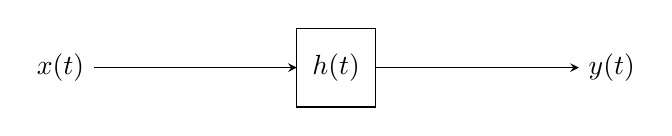
\begin{tikzpicture}
				\node (A) at (-3, 0) {\( x(t) \) };
				\node (B) at (4, 0) {\( y(t) \) };
				\draw[-stealth] (A) -- (0, 0);
				\draw (0, -0.5) rectangle node {\( h(t) \) } (1, 0.5);
				\draw[-stealth] (1, 0) -- (B);
			\end{tikzpicture}
		\end{center}
		Then, \( y(t) \), the signal generated by an arbitrary \( x(t) \) is generated by:
		\[
		y(t) = \int_{-\infty}^{\infty} x(\tau) h(t - \tau) \diff \tau 
		\] 
		In discrete time, the formula is: 
		\[
			y[n] = \sum_{k= -\infty}^{\infty} x[k] h[n - k]
		\] 
		This is called a \textit{convolution}, we will come back to this later. 
\end{itemize}
\subsubsection{Why a convolution?}
\begin{itemize}
	\item Again, consider the diagram:
	\begin{center}
			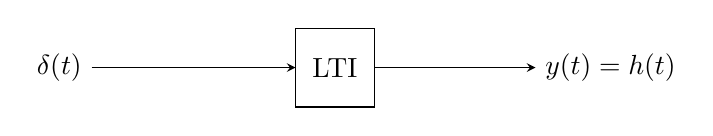
\begin{tikzpicture}
				\node (A) at (-3, 0) {\( \delta(t) \) };
				\node (B) at (4, 0) {\( y(t) = h(t)\) };
				\draw[-stealth] (A) -- (0, 0);
				\draw (0, -0.5) rectangle node {LTI } (1, 0.5);
				\draw[-stealth] (1, 0) -- (B);
			\end{tikzpicture}
		\end{center}
		If we send a signal \( \delta(t - \tau) \) into the system, then due to linear time invariance, the 
		system should output \( y(t - \tau) = h(t - \tau) \). 
	\item If we now send the signal \( x(\tau) \delta(t - \tau) \), then because \( x(\tau) \) is a constant, 
		then we invoke linearity to get that the output is  \( x(\tau) h(t - \tau) \). 
	\item Now, consider what happens when we send in the signal that is just a combination of all possible \( \tau \). 
		Each \( x(\tau) \) is a constant, so the output signal is of the form
		\[
		\int_{-\infty}^{\infty} x(\tau) \delta(t - \tau) \mapsto \int_{-\infty}^{\infty} x(\tau) h(t - \tau) 
		\diff \tau
		\] 
		But now notice that this signal can also be written as:
		\[
		\int_{-\infty}^{\infty} x(\tau) \delta(t - \tau) \diff \tau = x(t)
		\] 
		And so if we're sending in a signal \( x(t) \), then the output should be \( y(t) \)! Thus, we've proven that
		the impulse response is all we need in order to characterize \( y(t) \).
	\item For future reference, a convolution, denoted by \( x(t) * h(t) \), is defined as: 
		\[
		x(t) * h(t) = \int_{-\infty}^{\infty} x(\tau) h(t - \tau) \diff  \tau = \int_{-\infty}^{\infty} x(t - \tau)
		h(\tau) \diff \tau
		\] 
		this last equality shows that convolution is a commutative operation. 
\end{itemize}
\subsubsection{Impulse Response of 1st order LCCDE}
\begin{itemize}
	\item Recall the step response to LCCDE:
		\[
			\dv{y(t)}{t} + ay(t) = bx(t) = bu(t) \implies y_{\text{step}}(t) = 
			\left( \frac{b}{a}( 1 - e^{-at}) \right) u(t)
		\] 
	\item Given an impulse, which in this case can be written as: 
		\[
		\delta(t) = \lim_{\epsilon \to 0}\frac{u(t) - u(t - \epsilon)}{\epsilon}
		\] 
		This implies that the response \( h(t) \) is given by: 
		\[
		h(t) = \lim_{\epsilon \to 0 }\frac{y_{\text{step}}(t) - y_{\text{step}}(t - \epsilon)}{\epsilon} 
		= \lim_{\epsilon \to 0}
		\frac{\frac{b}{a}\left( e^{-a(t - \epsilon)}u(t - \epsilon) - e^{-at}u(t) \right) }{\epsilon}
		= be^{-at}u(t)
		\] 
		(verify this at home, the simplification makes use of the fact that \( e^{a\epsilon} \approx 
		1 + a\epsilon + a^2 \frac{\epsilon^2}{2} + \cdots\), but the higher order terms die).
\end{itemize}
\subsection{Harmonic Response of an LTI system}
\begin{itemize}
	\item The response of an LTI system to a complex signal \( x(t) = Ae^{j \omega t} \) is always going to be another 
		complex exponential signal \( y(t) = H(\omega) Ae^{j \omega t} \)
	\item Given the input signal \( x(t) = Ae^{j \omega t} \), we can write:
		\begin{align*}
			y(t) &= \int_{-\infty}^{\infty} x(\tau) h(t - \tau) \diff \tau\\
				 &= \int_{-\infty}^{\infty} Ae^{j \omega t}
			h(t - \tau) \diff \tau \\
				 &= \int_{-\infty}^{\infty} Ae^{j \omega (t - \tau')}h(\tau') \diff \tau'\\
				 &= Ae^{j \omega t}\underbrace{\int_{-\infty}^{\infty} e^{-j \omega \tau'}h(\tau') \diff \tau'}_{
				 H(\omega)}\\
				 &= H(\omega) Ae^{j \omega t} 
		\end{align*} 
	\item By definition:
		\[
		H(\omega) \equiv \int_{-\infty}^{\infty} e^{-j \omega \tau'}h(\tau') \diff \tau' \ \ 
		H(f) \equiv \int_{-\infty}^{\infty} e^{-j 2 \pi ft}h(t) \diff t 
		\] 
		You'll recognize \( H(\omega) \): it's the Fourier transform equation.
		
		\question{When given an harmonic input, and we're asked to measure it, are we measuring the real part 
		of the signal?}
\end{itemize}
\subsubsection{Example: Frequency response of an RC Circuit}
\begin{itemize}
	\item Given the following circuit:
		% insert circuitkkz
	\item The impulse response is given by the differential equation:
		\[
			\dv{y(t)}{t} + \frac{1}{RC}y(t) = \frac{1}{RC}x(t)
		\] 
		This is a first order LCCDE, so therefore the impulse response \( h(t) \) is given by 
		\( h(t) = be^{-at}u(t) \). 
	\item For the frequency response, we have a function of the form \( x(t) = e^{j \omega t} \), 
		which we know has an output signal of the form \( y(t) = H(\omega) e^{j \omega t} \). So all that remains
		now is to find \( H(\omega) \) :
		\begin{align*}
			y(t) &= e^{j \omega t }\int_{-\infty}^{\infty} e^{-j \omega t}h(\tau) \diff  \tau \\
			&= e^{j \omega t}\int_{-\infty}^{\infty} be^{-a\tau}u(\tau) e^{-j \omega \tau}\diff \tau  \\
			&= be^{j \omega t}\int_{0}^{\infty} e^{-a \tau}e^{-j \omega \tau}\diff \tau  \\
			&= \left( \left.-\frac{1}{a + j \omega}e^{-a \tau}e^{-j \omega t}\right|_0^{\infty}\right)
				be^{j \omega t} \\
				&= \frac{b}{a + j \omega}e^{j \omega t} 
		\end{align*}
		Now, if we impose that \( a = b = \frac{1}{RC} \), then we get the equation: 
		\[
		\frac{\frac{1}{j c \omega}}{\frac{1}{j c \omega} + R}e^{ j \omega t}
		\] 
		Now, \( \frac{1}{jc\omega} \) is the impedance of a capacitor, and this overall equation takes the form of a 
		voltage divider for a circuit with known impedance: 
		\[
		y(t) = \frac{z(\omega)}{z(\omega) + R}e^{j \omega t}
		\] 
\end{itemize}
\subsection{Sinusoidal Input} 
\begin{itemize}
	\item With the harmonic response tools, we can now evaluate the system response when given a sinusoidal 
		input, since we know that 
		\[
		\cos(\omega t) = \frac{e^{ j \omega t} + e^{- j \omega t}}{2}
		\] 
		\question{Does the same work with sine, where there's a complex number is in the denominator?} 
\end{itemize}
\subsection{LTI systems in Parallel and Series}
\begin{itemize}
	\item For a basic system with a single input and output, 
		we've already discussed that \( y(t) = x(t) * h(t) \). Now, what if we connect these systems in 
		parallel?
		\begin{center}
			\begin{tikzpicture}
				\node (A) at (-3, 0) {\( x(t) \) };
				\node (B) at (4, 0) {\( y(t) \) };
				\node (C) at (1.5, 0) {+};
				\draw[-stealth] (A) -- (-0.5, 0) -- (-0.5, 1) -- (0, 1);
				\draw (0, 0.5) rectangle node {\( h_1(t) \) } (1, 1.5);
				\draw[-stealth] (-0.5, 0) -- (-0.5, -1) -- (0, -1);
				\draw (0, -0.5) rectangle node {\( h_2(t) \) } (1, -1.5);
				\draw[-stealth] (1, 1) -- (1.5, 1) -- (C);
				\draw (C) circle (0.2cm);
				\draw[-stealth] (C) -- (B);
				\draw[-stealth] (1, -1) -- (1.5, -1) -- (C);
			\end{tikzpicture}
		\end{center}
		then, the result \( y(t) \) is given by \( y(t) = x(t) * h_1(t) + x(t) * h_2(t) = x(t) * 
		(h_1(t) + h_2(t))\).
	\item If we connect them in series: 
		\begin{center}
			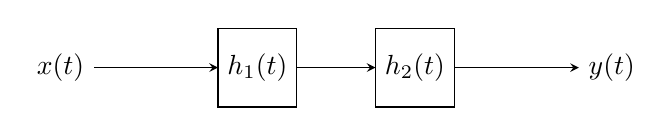
\begin{tikzpicture}
				\node (A) at (-3, 0) {\( x(t) \) };
				\node (B) at (4, 0) {\( y(t) \) };
				\draw[-stealth] (A) -- (-1, 0);
				\draw (-1, -0.5) rectangle node {\( h_1(t) \) } (0, 0.5);
				\draw[-stealth] (0, 0) -- (1, 0);
				\draw (1, -0.5) rectangle node { \( h_2(t) \) } (2, 0.5);
				\draw[-stealth] (2, 0) -- (B);
			\end{tikzpicture}
		\end{center}
		then	
\end{itemize}

	\section{Polynomial Multiplication II}
\begin{itemize}
	\item As a recap, we have two polynomials \( p \) and \( q \), both of degree \(  n -1 \), and we want to multiply 
		them. 
	\item We saw the \textit{coefficient representation}, where we specify its coefficients. So for \( p \), we have \( (p_0, p_1, 
		\dots, p_{n-1})\). Last lecture, we saw \( O(n^2) \) algorithm to multiply the polynomials using the 
		coefficient representation.
	\item We also saw the \textit{value representation}, where instead of giving the polynomial itself we give a set of 
		\( m \) points that the polynomial passes through. As long as \( m \ge  n \), then this set of points 
		fully specifies the polynomial. With this representation, we saw that polynomials can be multiplied in \( O(n) \) time. 
	\item So our main question was: is there a way for us to use the value representation to speed up the coefficient 
		representation multiplication?
	\item Roots of unity: the set of points we will evaluate our polynomials on. 
\end{itemize}
\subsection{Fast Fourier Transform}
\begin{itemize}
	\item Input: \( m \), a power of 2, a \( p(x) = p_0 + p_1x + \cdots + p_{m-1}x^{m-1} \). Our goal is to evaluate 
		 \( p( \omega_0), p(\omega_1), \dots, p(\omega_{m - 1}) \). 
	 \item We will use a divide and conquer approach:
		 \begin{center}
		 	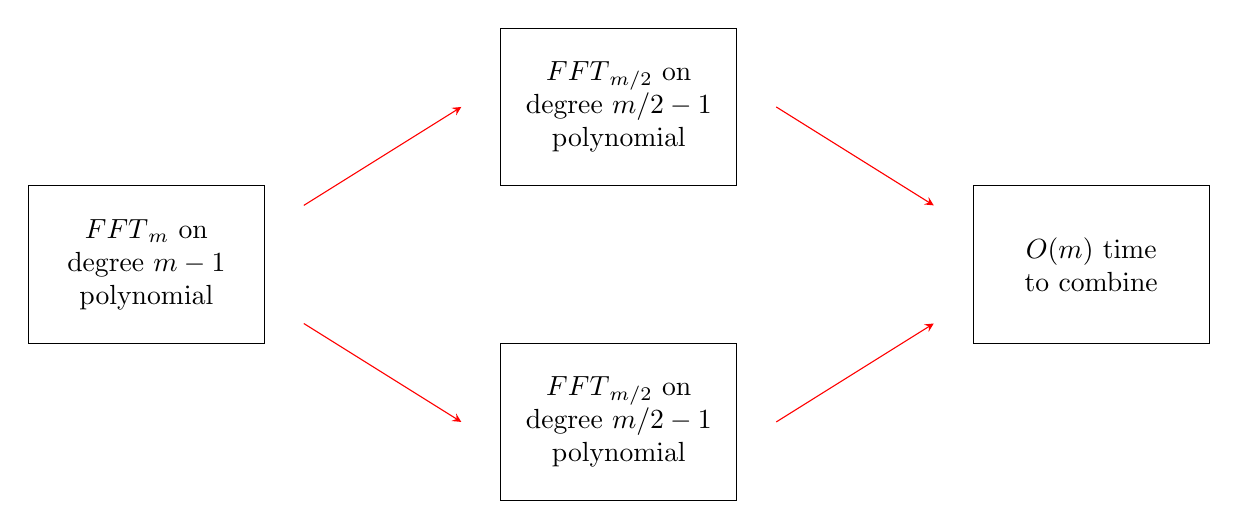
\begin{tikzpicture}[every text node part/.style={align=center}]
		 		\draw(0, -1) -- (3, -1) -- (3, 1) -- (0, 1) -- cycle;
				\draw(6, 1) -- (9, 1) -- (9, 3) -- (6, 3) -- cycle;
				\draw(6, -1) -- (9, -1) -- (9, -3) -- (6, -3) -- cycle;
				\draw(12, -1) -- (15, -1) -- (15, 1) -- (12, 1) -- cycle;
				\draw node at (1.5, 0) {\( \text{FFT}_m \) on \\degree \( m - 1 \) \\ polynomial}; 
				\draw node at (7.5, 2) { \( \text{FFT}_{m / 2} \) on \\ degree \( m / 2 - 1 \) \\ polynomial};
				\draw node at (7.5, -2) { \( \text{FFT}_{m / 2} \) on \\ degree \( m / 2 - 1 \) \\ polynomial};
				\draw node at (13.5, 0) {\( O(m) \) time \\ to combine};
				\draw[-stealth, red] (3.5, 0.75) -- (5.5, 2);
				\draw[-stealth, red] (3.5, -0.75) -- (5.5, -2);
				\draw[-stealth, red] (9.5, 2) -- (11.5, 0.75);
				\draw[-stealth, red] (9.5, -2) -- (11.5, -0.75); 
		 	\end{tikzpicture}
		 \end{center}
		 This will give us a recurrence relation \( T(m) \le  2 \cdot T(m / 2) + O(m) \), and from the master theorem this 
		 gives an \( O(m \log m) \) runtime.
\end{itemize}
\subsection{Divide and Conquer}
\begin{itemize}
	\item To figure out how to divide, let's first write out \( p(x) \) :
		\[
		p(x) = p_0 + p_1x + p_2x^2 + p_3x^3 + \cdots
		\] 
		Let's split \( p \) into two parts, based on the parity of the exponent. We'll call these the even and odd 
		halves:
		\begin{align*}
			p_E(x) &= p_0 + p_2x^2 + p_4x^{4} + \cdots + p_{m - 2}x^{m - 2}\\
			p_O(x) &= p_1x + p_3x^3 + \cdots + p_{m - 1} x^{m - 1} 
		\end{align*}
		But notice that we can rewrite the even part a little bit:
		\[
		p_E(x) = p_0 + p_2(x^2) + p_4(x^2)^2 + p_6(x^2)^3 + \cdots = \text{Even}(x^2)
		\] 
		But this looks like a polynomial with coefficietns \( p_0, p_2, p_4, \dots \) evaluated on \( x^2 \)! We will call 
		this polynomial \( \text{Even}(z) \). For the odd part, we factor out an \( x \) :
		\[
		p_1x + p_3x^3 + \cdots = x(p_1 + p_3x^2 + p_5x^{4} + \cdots) = x \cdot \text{Odd}(x^2)
		\] 
		The key to note here is that we have a recursion in the fact that we can express the evaluation of the polynomials 
		at the \( n \)-th step as a computation involving another polynomial but evaluated on \( x^2 \). So, we have 
		\[
		p(x) = \text{Even}(x^2) + x \cdot \text{Odd}(x^2)
		\] 
		The degree of the even part is \( (m - 2) / 2 = m / 2 - 1 \), and the same goes for odd part.   
	\item Now if we want to compute \( p \) on \( \omega_i \), then we have \( p(\omega_i) = \text{Even}(\omega_i^2) + 
		\omega_i \cdot \text{Odd}(\omega_i^2)\). 
	\item Because we are squaring the arguments, then this means that we are evaluating the Even and Odd parts on the 
		\( m / 2 \)-th roots of unity, because of our magical fact!
	\item So to compute \( p(\omega_i) \), we recursively evaluate the even and odd parts at the  \( m / 2 \)-th roots of unity:
		\( \alpha_0, \alpha_1, \dots, \alpha_{m / 2 - 1} \). 
	\item To combine, all we need to do is multiply the odd part by  \( \omega_i \), then add the two parts together. So, the 
		combination step only takes \( O(m) \) work. So this fully gives our recursion \( T(m) \le  2 \cdot T(m / 2) + O(m) \), 
		hence the \( O(m \log m) \) runtime. 
\end{itemize}
\subsection{Fast Interpolation}
\begin{itemize}
	\item An update on our algorithm scheme:
		\begin{center}
			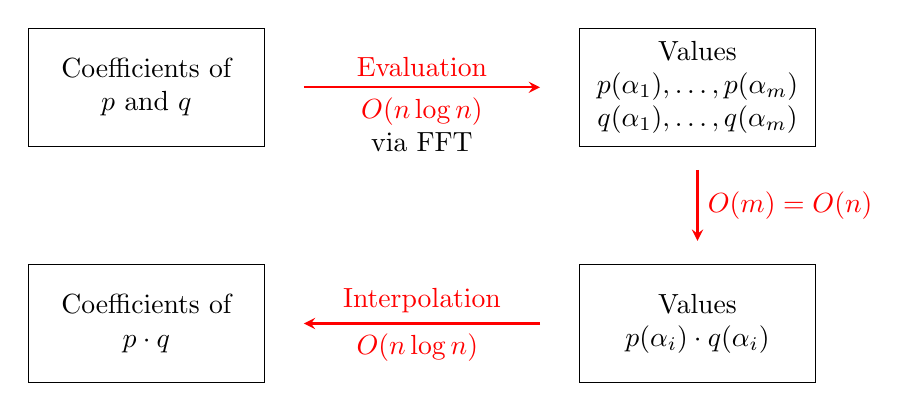
\begin{tikzpicture}[every text node part/.style={align=center}]
				\foreach \x in {0, 7}
				\foreach \y in {0, 3}
				{
					\draw (\x, \y) -- (\x+3, \y) -- (\x+3, \y+1.5) -- (\x, \y+1.5) -- cycle;
				}
				\draw node at (1.5, 0.75) {Coefficients of \\ \( p \cdot q \)};
				\draw node at (1.5, 3.75) {Coefficients of \\ \( p \) and \( q \) };
				\draw node at (8.5, 0.75) {Values \\ \( p(\alpha_i) \cdot q(\alpha_i) \) };
				\draw node at (8.5, 3.75) {Values \\ \( p(\alpha_1), \dots, p(\alpha_m) \) \\ \( q(\alpha_1), \dots, q(\alpha_m) \) };
				\draw[-stealth, red, thick] (3.5, 3.75) --node[midway, above] {Evaluation} node[midway, below] 
					{\( O(n \log n) \) \\ \textcolor{black}{via FFT}} (6.5, 3.75); 
				\draw[-stealth, red, thick] (8.5, 2.7) -- node[midway, right] {\( O(m) = O(n) \) } (8.5, 1.8);
				\draw[-stealth, red, thick] (6.5, 0.75) -- node[midway, above] {Interpolation} node[midway, below] 
					{\( O(n \log n) \) } (3.5, 0.75);
			\end{tikzpicture}
		\end{center}
	\item Now we want to figure out the interpolation step: given \( r(\omega_0), r(\omega_1), \dots, r(\omega_{m - 1}) \), we want 
		to get back the coefficient representation of \( r(x) \). This is called the inverse FFT. 
	\item It turns out that when we do the Fourier transform, we basically get the inverse Fourier transform for free. Recall 
		the Fourier transform:
		\[
			p(\omega_\ell) = \sum_{j = 0}^{m - 1}p_j (\omega_\ell)^{j}
		\]
		This equation comes from replacing all \( x \) 's with \( \omega_\ell \). Then, the inverse Fourier transform is written 
		as follows:
		\[
			p_{\ell} = \frac{1}{m} \cdot \sum_{j = 0}^{m - 1}p(\omega_j) \cdot (\omega_{m - \ell})^{j} = \frac{1}{m} \cdot 
			q(\omega_{m - \ell})
		\] 
		Here, \( q(x) = p(\omega_0) + p(\omega_1)x + \cdots p(\omega_{m - 1})x^{m - 1} \). So in essence, this is basically another 
		polynomial evaluation, which we already know happens in \( O(m \log m) = O(n \log n) \) time!
	\item So, now let's look at the completed diagram:
		\begin{center}
			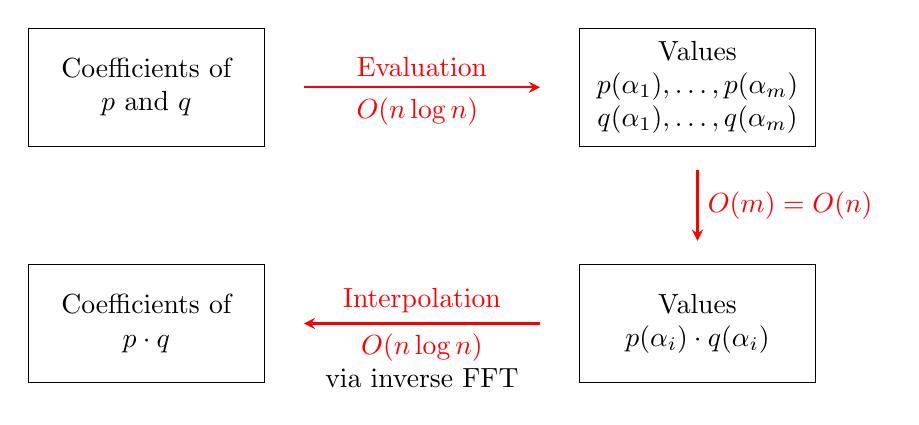
\begin{tikzpicture}[every text node part/.style={align=center}]
				\foreach \x in {0, 7}
				\foreach \y in {0, 3}
				{
					\draw (\x, \y) -- (\x+3, \y) -- (\x+3, \y+1.5) -- (\x, \y+1.5) -- cycle;
				}
				\draw node at (1.5, 0.75) {Coefficients of \\ \( p \cdot q \)};
				\draw node at (1.5, 3.75) {Coefficients of \\ \( p \) and \( q \) };
				\draw node at (8.5, 0.75) {Values \\ \( p(\alpha_i) \cdot q(\alpha_i) \) };
				\draw node at (8.5, 3.75) {Values \\ \( p(\alpha_1), \dots, p(\alpha_m) \) \\ \( q(\alpha_1), \dots, q(\alpha_m) \) };
				\draw[-stealth, red, thick] (3.5, 3.75) --node[midway, above] {Evaluation} node[midway, below] 
					{\( O(n \log n) \) } (6.5, 3.75); 
				\draw[-stealth, red, thick] (8.5, 2.7) -- node[midway, right] {\( O(m) = O(n) \) } (8.5, 1.8);
				\draw[-stealth, red, thick] (6.5, 0.75) -- node[midway, above] {Interpolation} node[midway, below] 
					{\( O(n \log n) \) \\ \textcolor{black}{via inverse FFT}} (3.5, 0.75);
			\end{tikzpicture}
		\end{center}
		So this shows that polynomial multiplication can be done in \( O(n \log n) \) time!  
\end{itemize}
\subsection{The Matrix Viewpoint}
\begin{itemize}
	\item There's another way to represent \( p(x) \), as a column vector:
		\[
		\begin{bmatrix} p(\omega_0)\\p(\omega_1)\\p(\omega_2)\\ \vdots \\ p(\omega_{m - 1}) \end{bmatrix} = 
		\begin{bmatrix} p_0 + p_1\omega_0 + p_2 \omega_0^2 + \cdots + p_{m-1}\omega_0^{m- 1}\\
		p_0 + p_1 \omega_1 + p_2\omega_1^2 + \cdots + p_{m-1}\omega_1^{m-1}\\
	\vdots \\
p_0 + p_1\omega_{m-1} + p_2\omega_{m-1}^2 + \cdots+ p_{m-1}\omega_{m-1}^{m-1}\end{bmatrix} 
= \underbrace{\begin{bmatrix} 1 & \omega_0 & \omega_0^2 & \dots & \omega_0^{m-1}\\
1 & \omega_1 & \omega_1^2 & \dots & \omega_1^{m-1}\\
1 & \omega_2 & \omega_2^2 & \dots & \omega_2^{m-1}\\
\vdots & \vdots & \vdots & \ddots & \vdots\\
1 & \omega_{m-1} & \omega_{m-1}^2 & \dots & \omega_{m-1}^{m-1}\end{bmatrix}}_{M} \cdot \underbrace{\begin{bmatrix} p_0\\p_1\\p_2\\ \vdots \\p_{m-1} \end{bmatrix}}_{[p]} 
		\] 
	\item If we didn't know FFT, then this computation is just a matrix multiplied by a vector, whihc would take \( O(m^2) \)  
		time. However, FFT basically gives us a way to compute this matrix in \( O(m \log m) \) time!

		Note also that this also solves this \textbf{without ever writing down \( M \) !} 
	\item The Inverse FFT looks much cleaner in this representation:
		\[
		M^{-1} \cdot \begin{bmatrix} p(\omega_0)\\p(\omega_1)\\p(\omega_2)\\ \vdots \\ p(\omega_{m-1}) \end{bmatrix} = 
		\begin{bmatrix} p_0\\p_1\\p_2\\ \vdots \\ p_{m-1} \end{bmatrix} 
		\] 
	\item For \( M \) specifically, we have \( M_{ij} = \omega_i^{j} = (\omega_1^{i})^{j} = \omega_1^{ij} \). Then, the inverse 
		is defined as: \( (M^{-1})_{ij} = \frac{1}{n} \cdot \omega_{m-i}^{j} \). 
\end{itemize}
\subsection{Applications}
\begin{itemize}
	\item \textbf{Cross Correlation:}
		Given the product of \( p(x) = p_0 + p_1x + p_2x^2 + p_3x^3 \) and \( q(x) = q_0 + q_1x + q_2x^2 + q_3x^3 \), the 
		coefficient on \( x^{i} \) in \( p(x) \cdot q(x) \) is
		\[
		p_0q_{i} + p_1q_{i-1} + \cdots + p_{i-1}q_{1} + p_{i}q_0
		\] 
		Now consider two arrays \( [p_0, p_1, p_2, p_3] \) and \( [q_3, q_2, q_1, q_0] \). Now let's stack them on top of each 
		other and take the dot product of the overlap. Depending on where they overlap, it actually corresponds to the coefficient 
		on some \( x^{i} \) in \( p(x) \cdot q(x) \).  
		\begin{center}
			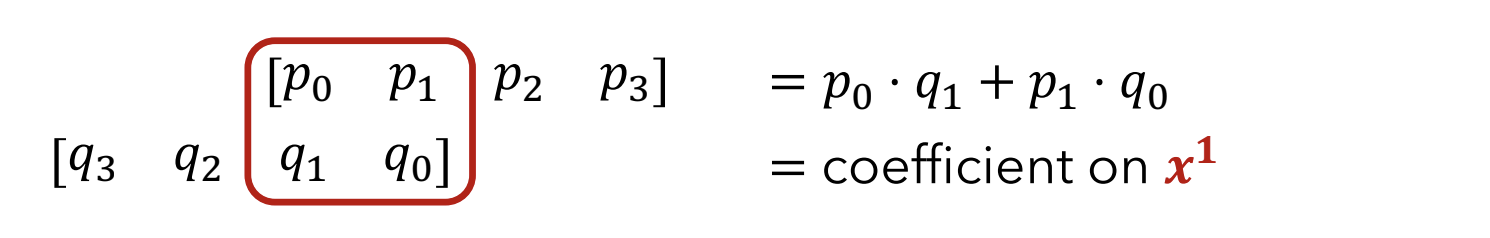
\includegraphics[scale=0.5]{cross-correlation.png}
		\end{center}
		This is called \textbf{cross-correlation}, and due to FFT, we can compute these in \( O(n \log n) \) time.   
	\item  \textbf{Integer Multiplication:} Say we wanted to multiply \( a = a_{n-1} \cdots a_2a_1a_0 \) and 
		\( b = b_{n-1}\cdots b_2b_1b_0 \). We can write down these two polynomials:
		\begin{align*}
			A &= a_0 + a_1x + a_2x^2 + \cdots + a_{n-1}x^{n-1}\\
			B&= b_0 + b_1x + b_2x^2 + \cdots + b_{n-1}x^{n-1} 
		\end{align*}
		and to compute the product, we can write \( A(x) \cdot B(x) \) and plug in \( x = 10 \). Naively we would think that 
		this takes \( O(n \log n) \) time, but this is not exactly true. This is because here, our additions and multiplications 
		don't exactly happen in \( O(1) \) time anymore, so we have to be careful! In fact, the multiplication can be as 
		large as \( \Theta(n) \). 

		After keeping track of all this, we get an \( O(n \log n \log \log n) \) algorithm. 
	\item \textbf{Fourier Transform:} FFT allows us to compute the Fourier transform of \( p(x) \) quickly -- we can decompose 
		 \( p(x) \) into its consistuent sines and cosines. There are too many applications of the Fourier transform to 
		 even list: 
		 \begin{enumerate}[label=\arabic*.]
		 	\item Music software
			\item Heart rate monitor
			\item Signal processing (e.g. cell phones)
			\item Many more!
		 \end{enumerate}
		 The fact that quantum computers can compute Fourier transforms exceedingly quickly is actually one of the main reasons 
		 that makes them so powerful.
\end{itemize}

	\section{Lecture 6}
\subsection{Clarification on BIBO Stability}
\begin{itemize}
	\item When we say a "bounded" signal, we mean that the amplitude of the signal is bounded at all times:
		\[
		|x(t)| < \infty \ \forall t \in \R
		\] 
		The same definition follows for discrete-time signals. 
	\item For LTI systems, we call the system BIBO stable if and only if its impulse \( h(t) \) is absolutely 
		integrable:
		\[
		\int_{-\infty}^{\infty} |h(t)| \diff t < \infty
		\] 
\end{itemize}
\subsection{Cross-Correlation}
\begin{itemize}
	\item The cross correlation between two signals \( r_{xy}(t) = r_{yx}(-t) \). To show this explicitly, we 
		look at the cross-correlation equation:
		\begin{align*}
			r_{xy}(t) &= \int_{-\infty}^{\infty} x(\tau)y(t + \tau) \diff \tau \\
			r_{yx}(t) &= \int_{-\infty}^{\infty} y(\tau) x(t + \tau) \diff \tau  
	\end{align*} 
	But for the second equation, we can define a \( \tau' = t + \tau\), so then we get: 
	\[
	r_{yx}(t) = \int_{-\infty}^{\infty} y(\tau' - t)x(\tau') \diff \tau' = \int_{-\infty}^{\infty} 
	x(\tau') y(-t + \tau') \diff \tau'
	\] 
	This looks like the first equation except we have \( -t \) instead of \( t \). Therefore, we have 
	\( r_{xy}(t) = r_{yx}(-t) \). The same works for discrete time: \( r_{xy}[n] = r_{yx}[-n] \). 
\end{itemize}

\subsection{More Convolution Properties} 
\begin{itemize}
	\item \textbf{Differentiation property:} Given \( y(t) = x(t) * h(t) \), then:
		\[
			\dv{t} y(t) = x(t) * \dv{h(t)}{t} = \dv{x(t)}{t} * h(t)
		\] 
	\item \textbf{Intergration Property:} Given \( y(t) = x(t) * h(t) \), we have:
		\[
		\int_{-\infty}^{t'} y(t) \diff  t = x(t) * \int_{-\infty}^{t'} h(\tau)\diff \tau 
		\] 
\end{itemize}
\subsection{Fourier Transform} 
\begin{itemize}
	\item The fourier transform came from the study of the heat equation, written as:
		\[
			c \rho \pdv{t} u(x, y, z, t) = k \left( \pdv[2]{x} + \pdv[2]{y} + \pdv[2]{z} \right) 
			u(x, y, z, t)
		\] 
		Fourier then claimed that the solution can be expanded in a series of sines with multiples of the variable. 
		In other word,s the solution is of the form:
		\[
		f(x) = \frac{1}{2a_0} + (a_1 \sin(x) + b_2 \cos(x)) + (a_2\sin(2x) + b_2\cos(2x)) + \cdots 
		\] 
	\item Recall the frequency response of an LTI system:
		\begin{center}
			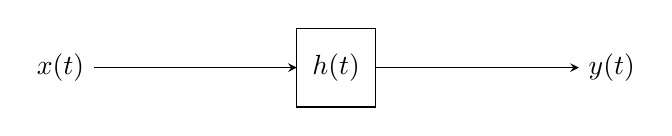
\begin{tikzpicture}
				\node (A) at (-3, 0) {\( x(t) \) };
				\node (B) at (4, 0) {\( y(t) \) };
				\draw[-stealth] (A) -- (0, 0);
				\draw (0, -0.5) rectangle node {\( h(t) \) } (1, 0.5);
				\draw[-stealth] (1, 0) -- (B);
			\end{tikzpicture}
		\end{center}
		Recall that we can characterize \( y(t) \) via a convolution: 
		\[
		y(t) = \int_{-\infty}^{\infty} x(\tau) h(t - \tau) \diff  \tau 
		\] 
		If we do this with our input \( e^{j 2 \pi ft} \), then we get:
		\[
		y(t) = H(f) e^{j 2 \pi ft} = H(\omega) e^{j \omega t }
		\] 
		Here, \( H(\omega) \) is defined to be the Fourier transfrm of the impusle response \( h(t) \):
		\[
			H(\omega) = \int_{-\infty}^{\infty} e^{- j \omega t} h(t) \diff t 
		\] 
		Alternatively, written in frequency language:
		\[
		H(f) = \int_{-\infty}^{\infty} e^{-j 2 \pi ft}h(t) \diff t 
		\] 
	\item Formally, the Fourier transform is defined as:
		\[
		H(f) \equiv \mathcal F \{h(t)\} \equiv \int_{-\infty}^{\infty} h(t) e^{-j 2\pi ft }\diff  t 
		\] 
		This transforms the signal \( h(t)  \) from the time domain into the frequency domain. The reason for this 
		is becuase the Fourier transform is a definite integral, which kills off any \( t \) dependence entirely. 
		In terms of angular frequency, we have:
		\[
		H(\omega) \equiv \mathcal F \{h(t)\} = \int_{-\infty}^{\infty} h(t) e^{-j \omega t}\diff t 
		\] 
	\item The inverse Fourier transform is:
		\[
			h(t) = \mathcal F^{-1} \{H(f)\} = \int_{-\infty}^{\infty} H(f) e^{j 2\pi ft}\diff  f 
		\]
		Since the Fourier transform takes objects from the time domain to the frequency domain, the inverse 
		Fourier transform takes things from the frequency domain to the time domain. 

		In terms of angular frequency, we have:
		\[
		h(t) = \mathcal F^{-1} \{H(\omega)\} = \frac{1}{2\pi}\int_{-\infty}^{\infty} H(\omega) 
		e^{j \omega t}\diff \omega 
		\] 
		This is also sometimes called the "synthesis equation", since we basically create \(  x(t) \) out of 
		\( H(\omega) \). 
	\item We can also provably show that the Inverse fourier transform does indeed invert the Fourier transform, 
		albeit with a lot of algebra. See lecture slides for the full derivation.  
	\end{itemize}

\end{document}
